%!TeX root=../tese.tex
%("dica" para o editor de texto: este arquivo é parte de um documento maior)
% para saber mais: https://tex.stackexchange.com/q/78101/183146

%% ------------------------------------------------------------------------- %%
\chapter{Árvores splay}
\label{cap:arvores-splay}

Neste capítulo apresentaremos a estrutura Árvore Splay desenvolvida por \cite{selfadjustingbst}. Descreveremos a implementação e funcionamento das operações splay, acess, insert, delete, split e join e analisaremos o custo amortizado da árvore.


\section{Introdução}
O algoritmo tradicional de busca em ABB inicia a execução de um acesso na raiz e desce para o filho apropriado até alcançar a chave procurada. O pior caso é quando a chave procurada está em um nó folha mais profundo. Nesse caso, o algoritmo tem que passar por toda a altura da árvore até chegar a essa folha. Assim o custo do pior caso é proporcional à altura da árvore que, no pior dos casos é linear $\mathcal{O}(n)$ e no melhor dos casos, tem custo $\mathcal{O}(\log{}n)$.

Com base neste limitante inferior de custo $\Omega(\log{}n)$ para buscas em ABBs, foram desenvolvidas uma série de estruturas conhecidas como \textit{árvores binárias de busca balanceadas}. Essas árvores têm o intuito de minimizar a própria altura por meio de rotações e consequentemente mitigar o custo de acessos de pior caso. Muitas dessas estruturas também se utilizam de armazenamento de memória adicional por nó para manter informações essenciais para a lógica de balanceamento proposta. 

Apesar dessas estruturas serem bastante eficientes, tendo tempo por busca logarítmico no número de elementos, elas não conseguem alcançar uma eficiência superior a isso independente da entrada. Padrões de acesso do mundo real muitas vezes possuem tendências ou estruturas repetitivas, como por exemplo bancos de dados que recebem solicitações frequentes para um pequeno número de elementos de alto tráfego. Em alguns desses casos, é possível ter uma performance melhor que $\mathcal{O}(\log{}n)$ mesmo com um algoritmo de busca online.

Uma alternativa para uma performance melhor é a árvore splay. Árvore Splay é uma árvore binária de busca balanceada proposta por \cite{selfadjustingbst}. Diferentemente das árvores binárias balanceadas citadas anteriormente, a árvore splay se reestrutura após cada operação, inclusive após acessos e não utiliza armazenamento adicional.

A árvore splay é uma ABB que segue a heurística “move to front”, ou seja, a ideia central é que a medida que operações são realizadas na estrutura, os elementos são movidos para perto da raiz de uma maneira particular com intuito de manter na raiz o último nó acessado.
Com a tendência dos nós mais recentemente acessados estarem próximos da raiz, o custo de sequências de acessos repetitivos tende a diminuir e essas reestruturações também auxiliam a árvore splay a dispor seus nós de maneira mais balanceada, reduzindo a altura total da árvore em alguns casos.

\section{Operação Splay}

A essência da árvore splay está na operação splay A operação splay é a responsável por mover um nó específico para a raiz por meio de rotações sucessivas. Essa operação é fundamental para o funcionamento da estrutura e é utilizada por todas as outras operações.

A operação splay se utiliza de três tipos distintos de rotações para trazer um nó para a raiz: zig, zig-zig e zig-zag.

Seja $x$ o nó interno a ser deslocado para a raiz. 

\subsection{Caso zig}

A rotação zig acontece quando $x$ é descendente direto do nó raiz. Neste caso apenas é necessário realizar uma rotação no nó $x$ e $x$ se encontrará na raiz da árvore.

\begin{figure}[h]
    \centering
    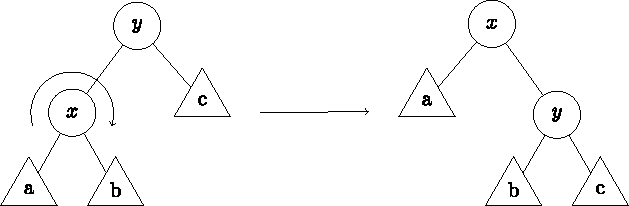
\includegraphics{images/zig.pdf}
    \label{fig:zig}

\caption{Caso zig com $x$ nó esquerdo da raiz.}
\end{figure}

\subsection{Caso zig-zig}

A rotação zig-zig acontece quando $x$ e seu pai são ambos filhos direitos ou ambos filhos esquerdos. Neste caso, é necessário rotacionar o pai de $x$ primeiro e em seguida rotacionar $x$.

\begin{figure}[h]
    \centering
    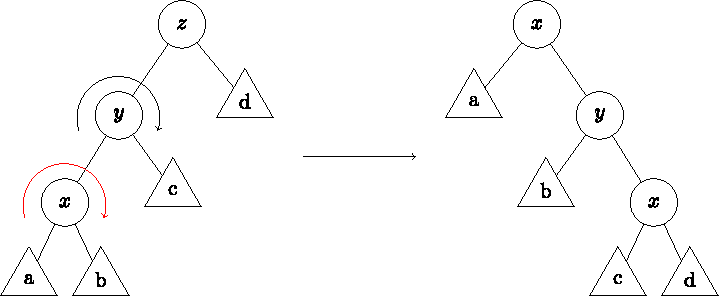
\includegraphics{images/zigzig.pdf}
    \label{fig:zigzig}

\caption{Caso zig-zig com $x$ e $y$ filhos esquerdos. A flecha preta e a vermelha representam respectivamente as rotações a serem realizadas em primeiro e por último.}
\end{figure}

\subsection{Caso zig-zag}

A rotação zig-zag acontece quando $x$ e seu pai não são ambos filhos direitos ou ambos filhos esquerdos. Neste caso, é necessário rotacionar $x$ duas vezes. Vale ressaltar que cada rotação será feita para um lado.
%\begin{figure}[hbt!]
%\centering
%\begin{tikzpicture}[
%ed/.style = {densely dashed, shorten >= 5pt},
%alpha/.style = {regular polygon, regular polygon sides=3, draw, minimum size=1.1cm, inner sep=2pt, anchor=south},
%level distance=1.5cm,
%sibling distance=0.25cm 
%]
%\begin{scope}[local bounding box=scope1]
%    \Tree [.$z$  [.$y$ \node[alpha]{a}; [.$x$ \node[alpha]{b}; \node[alpha]{c}; ]] \node[alpha]{d};]
%\end{scope}

%\begin{scope}[xshift=6cm, local bounding box=scope2, scale=1, level distance=2.25cm, sibling distance=0.25cm]
%    \Tree [.$x$ [.$y$ \node[alpha]{a}; \node[alpha]{b};] [.$z$  \node[alpha]{c}; \node[alpha]{d};]]]
%\end{scope}

%\draw[->] ([yshift=-0.5*\ht\strutbox,xshift=0.5cm]scope1.east) -- node {} ([yshift=-0.5*\ht\strutbox,xshift=-0.1cm]scope2.west); 

%\draw[->] ([yshift=-3.67cm, xshift=0.67cm]scope1.north) arc (-18:198:0.7cm);
%\draw[->,red] ([yshift=-3.67cm, xshift=-0.78cm]scope1.north) arc (198:-18:0.82cm);

%\end{tikzpicture}

\begin{figure}[h]
    \centering
    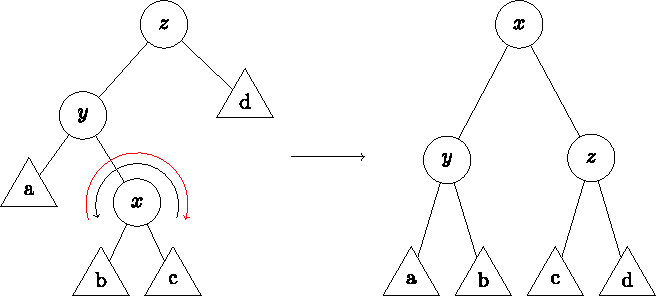
\includegraphics{images/zigzag.pdf}
    \label{fig:zigzag}

\caption{Caso zig-zag com $x$ filho direito e $y$ filho esquerdo. A flecha preta e a vermelha representam respectivamente as rotações a serem realizadas em primeiro e por último.}
\end{figure}
